%%%% Proceedings format for most of ACM conferences (with the exceptions listed below) and all ICPS volumes.
\documentclass[sigconf]{acmart}
\usepackage{algorithm}
\usepackage[export]{adjustbox}
\usepackage[noend]{algpseudocode}
\usepackage{todonotes}
\usepackage{xspace}
%%%% As of March 2017, [siggraph] is no longer used. Please use sigconf (above) for SIGGRAPH conferences.

%%%% Proceedings format for SIGPLAN conferences 
% \documentclass[sigplan, anonymous, review]{acmart}

%%%% Proceedings format for SIGCHI conferences
% \documentclass[sigchi, review]{acmart}

%%%% To use the SIGCHI extended abstract template, please visit
% https://www.overleaf.com/read/zzzfqvkmrfzn

%
% defining the \BibTeX command - from Oren Patashnik's original BibTeX documentation.
\def\BibTeX{{\rm B\kern-.05em{\sc i\kern-.025em b}\kern-.08emT\kern-.1667em\lower.7ex\hbox{E}\kern-.125emX}}
    
% Rights management information. 
% This information is sent to you when you complete the rights form.
% These commands have SAMPLE values in them; it is your responsibility as an author to replace
% the commands and values with those provided to you when you complete the rights form.
%
% These commands are for a PROCEEDINGS abstract or paper.
\copyrightyear{2019}
\acmYear{2019}
\setcopyright{licensedusgovmixed}
\acmConference[EuroMPI '19]{EuroMPI '19: ACM International Conference Proceeding Series}{September 11th-13th, 2019 }{Zurich, Switzerland}
\acmPrice{15.00}
\acmDOI{10.1145/1122445.1122456}
\acmISBN{978-1-4503-9999-9/18/06}

%
% These commands are for a JOURNAL article.
%\setcopyright{acmcopyright}
%\acmJournal{TOG}
%\acmYear{2018}\acmVolume{37}\acmNumber{4}\acmArticle{111}\acmMonth{8}
%\acmDOI{10.1145/1122445.1122456}

%
% Submission ID. 
% Use this when submitting an article to a sponsored event. You'll receive a unique submission ID from the organizers
% of the event, and this ID should be used as the parameter to this command.
%\acmSubmissionID{123-A56-BU3}

%
% The majority of ACM publications use numbered citations and references. If you are preparing content for an event
% sponsored by ACM SIGGRAPH, you must use the "author year" style of citations and references. Uncommenting
% the next command will enable that style.
%\citestyle{acmauthoryear}

%
% end of the preamble, start of the body of the document source.
\begin{document}

%
% The "title" command has an optional parameter, allowing the author to define a "short title" to be used in page headers.
\title{Runtime level failure detection and propagation in HPC systems}

%
% The "author" command and its associated commands are used to define the authors and their affiliations.
% Of note is the shared affiliation of the first two authors, and the "authornote" and "authornotemark" commands
% used to denote shared contribution to the research.
\author{Dong Zhong
\orcid{1234-5678-9012}}
\email{dzhong@vols.utk.edu}
\affiliation{%
  \institution{The University of Tennessee}
  \streetaddress{1122 Volunteer Blvd}
  \city{Knoxville}
  \state{TN}
  \postcode{37996}
  \country{USA}
}
\author{Aurelien Bouteiller
\orcid{0000-0001-5108-509X}}
\email{bouteill@icl.utk.edu}
\affiliation{%
  \institution{The University of Tennessee}
  \streetaddress{1122 Volunteer Blvd}
  \city{Knoxville}
  \state{TN}
  \postcode{37996}
  \country{USA}
}
\author{George Bosilca
\orcid{0000-0003-2411-8495}}
\email{bosilca@icl.utk.edu}
\affiliation{%
  \institution{The University of Tennessee}
  \streetaddress{1122 Volunteer Blvd}
  \city{Knoxville}
  \state{TN}
  \postcode{37996}
  \country{USA}
}
%\author{Jack J. Dongarra}
%\orcid{0000-0003-3247-1782}
%\email{dongarra@icl.utk.edu}
%\affiliation{%
%  \institution{The University of Tennessee}
%  \streetaddress{1122 Volunteer Blvd}
%  \city{Knoxville}
%  \state{TN}
%  \postcode{37996}
%  \country{USA}
%}
%
% By default, the full list of authors will be used in the page headers. Often, this list is too long, and will overlap
% other information printed in the page headers. This command allows the author to define a more concise list
% of authors' names for this purpose.
%\renewcommand{\shortauthors}{Zhong, Bouteiller, et al.}

%
% The abstract is a short summary of the work to be presented in the article.
\begin{abstract}
TODO : fix the expression and maybe the logic ?
As the scale of High Performance Computing (HPC) system continues to grow, with more and more nodes deployed, mean-time-to-failure (MTTF) of those HPC systems is dramatic impacted (become lower and lower/drops). In order to efficiently run long time computing job on these systems, fault tolerance become a prime challenge/technology. In this paper, we present the design and implementation of an efficient runtime-level failure detection and propagation strategy targeting exascale systems. The detection is able to detect both node failure and process failure. A ring topology is maintained by allowing one node sending and receiving periodically heartbeat to/from another node to detect a node failure(observing another single node). For process failure each host node (is in charge of monitoring) monitors its children processes. The propagation use a reliable broadcast method over a binomial graph(an arbitrary communication topology) to distribute error message to applications, guarantees a logarithmic propagate time. We focus primarily on the most widely used programming paradigms PMIx Reference RunTime Environment(PRRTE), the algorithms and strategies proposed have a larger scope of most distributed programming environment. Experiments on different machines successfully demonstrated the algorithm performs well.
\end{abstract}

%
% The code below is generated by the tool at http://dl.acm.org/ccs.cfm.
% Please copy and paste the code instead of the example below.
%
\begin{CCSXML}
<ccs2012>
<concept>
<concept_id>10010520.10010521.10010537</concept_id>
<concept_desc>Computer systems organization~Distributed architectures</concept_desc>
<concept_significance>500</concept_significance>
</concept>
<concept>
<concept_id>10010520.10010521.10010542.10010546</concept_id>
<concept_desc>Computer systems organization~Heterogeneous (hybrid) systems</concept_desc>
<concept_significance>300</concept_significance>
</concept>
<concept>
<concept_id>10010520.10010575.10010577</concept_id>
<concept_desc>Computer systems organization~Reliability</concept_desc>
<concept_significance>300</concept_significance>
</concept>
<concept>
<concept_id>10010520.10010575.10011743</concept_id>
<concept_desc>Computer systems organization~Fault-tolerant network topologies</concept_desc>
<concept_significance>300</concept_significance>
</concept>
<concept>
<concept_id>10011007.10010940.10011003.10011005</concept_id>
<concept_desc>Software and its engineering~Software fault tolerance</concept_desc>
<concept_significance>300</concept_significance>
</concept>
<concept>
<concept_id>10011007.10011006.10011041.10011048</concept_id>
<concept_desc>Software and its engineering~Runtime environments</concept_desc>
<concept_significance>300</concept_significance>
</concept>
</ccs2012>
\end{CCSXML}

\ccsdesc[500]{Computer systems organization~Distributed architectures}
\ccsdesc[300]{Computer systems organization~Heterogeneous (hybrid) systems}
\ccsdesc[300]{Computer systems organization~Reliability}
\ccsdesc[300]{Computer systems organization~Fault-tolerant network topologies}
\ccsdesc[300]{Software and its engineering~Software fault tolerance}
\ccsdesc[300]{Software and its engineering~Runtime environments}

%
% Keywords. The author(s) should pick words that accurately describe the work being
% presented. Separate the keywords with commas.
\keywords{fault tolerance, failure detection, reliable broadcast, message propagation, HPC runtime system}

%
% This command processes the author and affiliation and title information and builds
% the first part of the formatted document.
\maketitle

\section{Introduction}
The drive to produce more and more powerful supercomputers leads to HPC platforms/systems consist millions of cores distributed over hundreds of thousands of nodes, it is becoming increasingly imperative to adopt fault tolerance and resilient features to applications and runtime environments. Efforts toward fault tolerance has been attempted by researchers at application level. 

A runtime environment support distributed HPC applications operating in heterogeneous environment, the system provide service for managing processes launching, deployment and monitoring, also providing interaction and communication infrastructures for hosts and parallel applications. 

A resilient runtime environment must have the capability of continuing the job execution even with failures, and also be able to detect failure and distribute the fault information to the applications with minimal disturbance to the whole system.  

TODO:
Detection and propagation ?

\section{Related work}
In this section, we survey related work on large scale distributed runtime environments,different kinds of heartbeat based and random gossip based failure detectors, together with reliable broadcast algorithms to propagate fault information.

\subsection{Runtime systems}
A wide range of approach to the problem of exscale distributed computing runtime environments have been studied, each primarily emphasizing a particular key aspect of the over all problem. MPICH provides several runtime environments, such as MPD\cite{Butler00}, Hydra and Gforker\cite{MPICH14}. MPD connects nodes through a ring topology which is not resilient, two node failures could separate nodes into two separates groups that prevents communication with one another. Another drawback is that this approach has proved to be non-scalable. Hydra scales well for large number of processes on a single node and efficient interaction with hybrid programming models that combine MPI and threads. The Open MPI runtime environment, ORTE\cite{Castain05}\cite{Jeffrey12} provides not only the required message passing API, but also an accompanying runtime system to launch, monitor, and kill parallel jobs. Also ORTE connect daemons through various topology, however the communication is not reliable. Also, all those runtimes are limited to MPI application.

PRRTE work has the capability to run MPI jobs more scalability, and also supports applications utilize more than one programming model, such as an MPI application that also uses OpenMP. 

\subsection{Failure detection}
Research in the ares of failure detection has been extensively studied. Chandar and Toueg\cite{Chandra96} proposed the first unreliable failure detector oracle that could solve consensus and atomic broadcast problem for reliable distributed systems. Many implementations\cite{Wei02}\cite{Larrea00}\cite{Kawazoe97} based on this oracle work are using all-to-all communication where every node periodically sends heartbeats to all nodes. However, those implementations are not scalable for lager systems with hundreds of thousands of nodes. The technique gossip-style protocols\cite{van98} \cite{Ranganathan01}\cite{Gupta01}\cite{Abhinandan02}  (where nodes pick some other nodes to monitor and exchange information) become popular approach for failure detection in order to scale up. However, gossip methods do not work well with large number node crashes, also detecting a specific failure could potentially take a fairly long time. Furthermore, gossip methods still have the disadvantage of redundant failure messages that decreases the scalability.

Recently, our previous work \cite{George18} proposed a observation ring based detector for HPC system,the simulation results demonstrate the efficient of the algorithm, however the implementation in ULFM is an application level failure detection strategy, which can only detect process failures. This extension resilient PRRTE work exceed the limitation and has the capability to detect both process and node failures which is also not limited to run MPI application only. 

\subsection{Reliable broadcast}
Notable efforts have been made for fault-tolerant communication based on existing logical network topologies. Fully connected topology is perfect in the sense of fault tolerant but cannot be scalable. A circular topology is good for scalability but suffers from multiple node failures.  
A more recent effort to introduce is k-nomial Graph \cite{Angskun07}\cite{Pava11}, the key-concept of fault-tolerant broadcasting is diameter of the topology, which is defined the longest shortest path between any two nodes in the graph. Binomial Graph has scalable capability properties with reasonable degree, regular graph and lowest diameter. However when doing a reliable broadcast with message forwarding, this method uses a fixed sending sequence to all the neighbours which has the disadvantage of not using high sending priority to unnotified nodes. Our work uses Binomial Graph with a reordering strategy when sending and forwarding messages, which means lower average reroute hops and message traffic density.

\section{Design and implementation}

In this section, we describe the design of Resilient PRRTE, our resilient mechanism has two components: a node level observation ring and a reliable broadcast overlay network. We also provide rationale for our design decisions,and detailed implementation.

\begin{figure}[h]
  \centering
  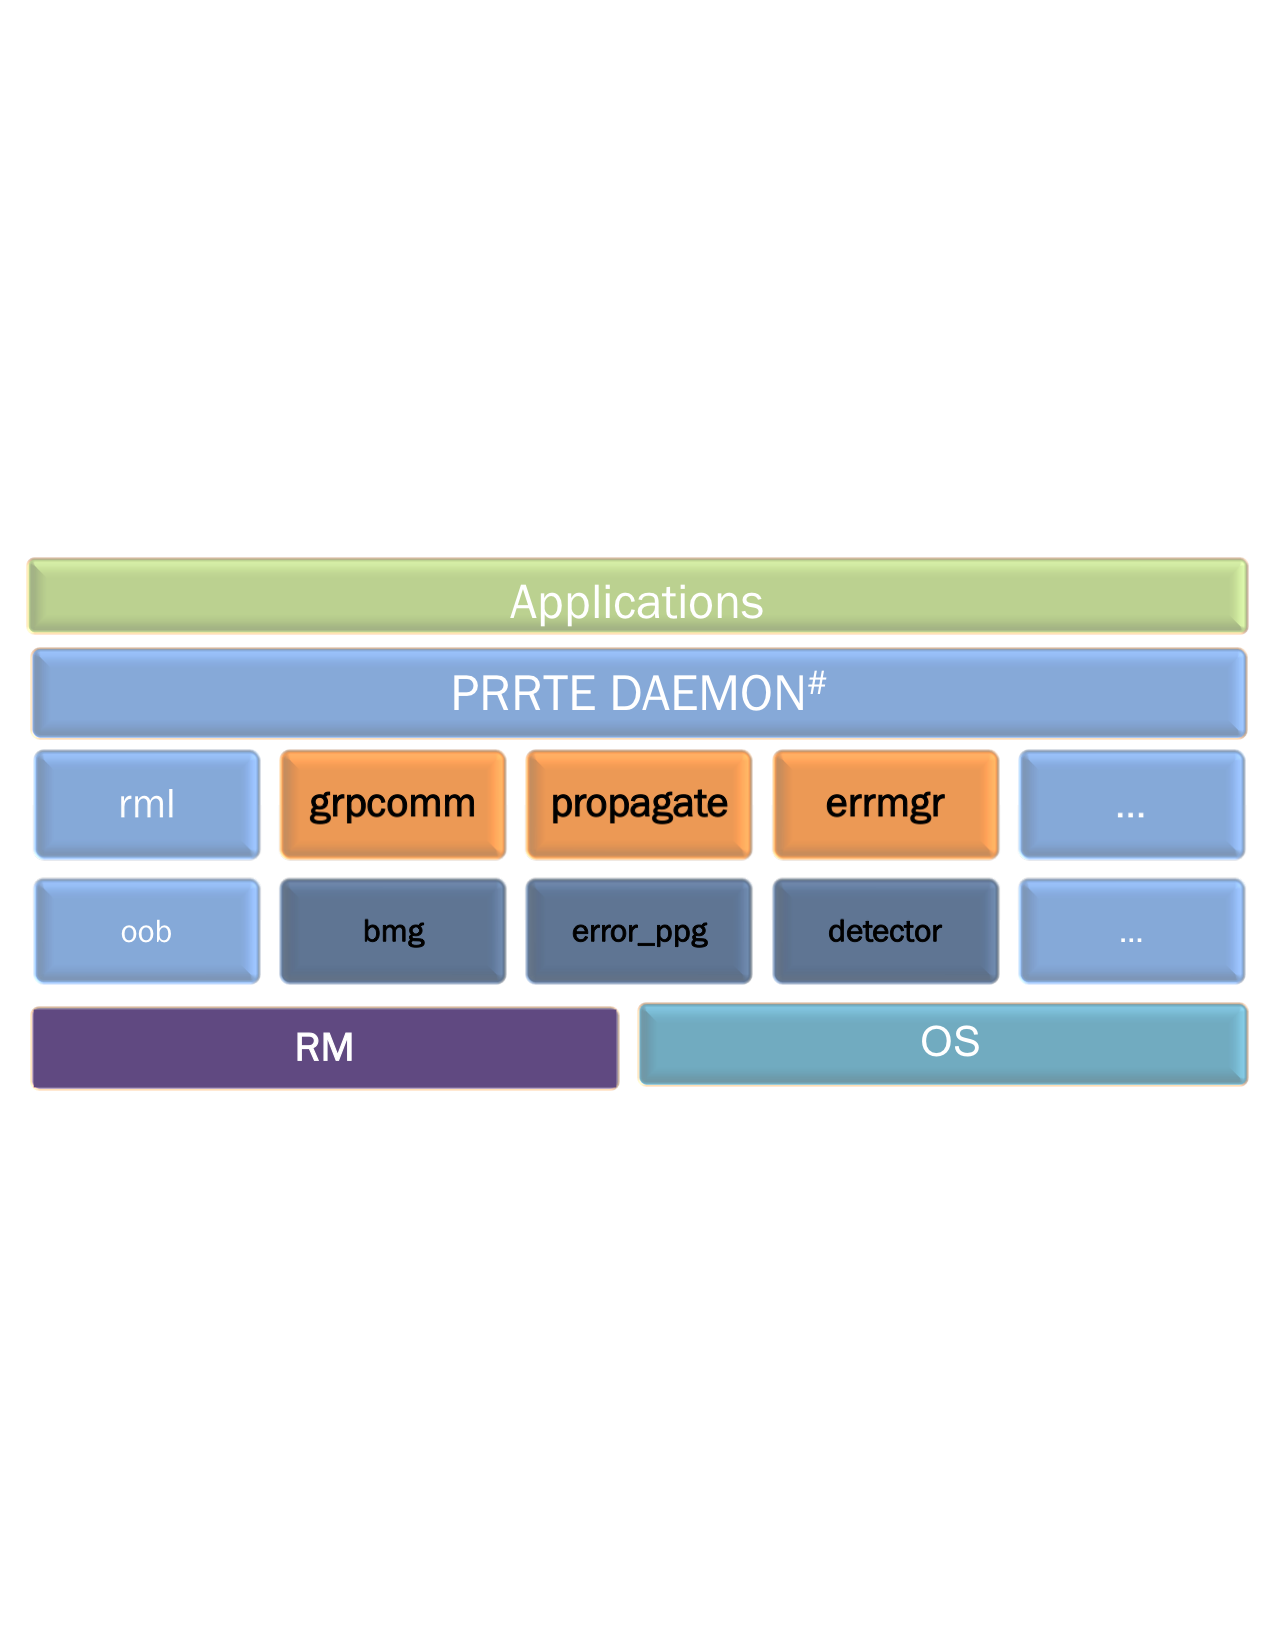
\includegraphics[trim=0.2cm 9.0cm 0.2cm 9cm,width=\linewidth]{PMIx_PRRTE.pdf}
  \caption{Resilient PRRTE component architecture. The orange boxes represent the component we mainly use to add the resilient features. The dark blue colored boxes are the new modules}
\end{figure}

\begin{figure}[h]
  \centering
  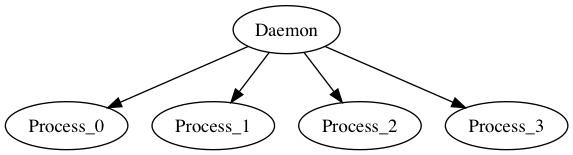
\includegraphics[width=\linewidth]{test.png}
  \caption{Notify the error locally}
\end{figure}
\subsection{Model}
PRRTE originated as OpenRTE \cite{Castain05} which is based upon Module Component Architecture (MCA) developed under the Open MPI project. As in figure 1, within this architecture, each of the major subsystems is defined as a MCA framework with well-defined interface. Also each framework contains one or more components each representing a different implementation. Then the OpenRTE work spun off to its own effort as a ``\verb|shim|`` between the application and the host environment that includes full support for the PMIx \cite{CASTAIN18} - an abstract set of interfaces by which not only applications and tools can interact with the resident system management stack (SMS), but also the various SMS components can interact with each other. 

PRRTE provides an easy way of launching, running and monitoring PMIx-based applications outside of a PMIx-enabled environment on distributed systems. The PRRTE overall architecture is out the scope of this paper, but we still want to mention some feature embraced by it. First of all, PRRTE's very first feature is Job controlling and Monitoring \cite{Ralph15} which enables the application and SMS to coordinate the response to failure: termination of the job or a subset of processes, request replacement of nodes and processes, or continue execution at a lower setting. This provides the foundation of resilience strategy of our work. Another important feature is the PMIx Event Notification \cite{Ralph002} : the resource manager or server can notify the application of events, the application processes can notify their server or SMS of issues. This provides the channel for locally propagation of error messages. Resilient PRRTE mainly embraces two new features of failure detection and reliable broadcast for messages propagation globally and locally. We will give a detail introduction of the two features in the following sections.

\subsection{Detection of process and node failure/Error management}

\begin{table}
  \caption{Parameters and notations}
  \label{tab:parameters}
  \begin{tabular}{ccl}
    \toprule
    Symbol & Description \\
    \midrule
    \texttt{\bf N} & Number of Daemon/nodes \\
    \texttt{Id} & The identifier of a Daemon \\
    \texttt{LIST\{ID\}} & List of known failed daemons' ID \\
    $\delta$ & Heartbeat period \\
    $\eta$ & Timeout for assuming a daemon failure\\
    \bottomrule
  \end{tabular}
\end{table}

\begin{figure}
\centering
\begin{minipage}{.23\textwidth}
  \centering
  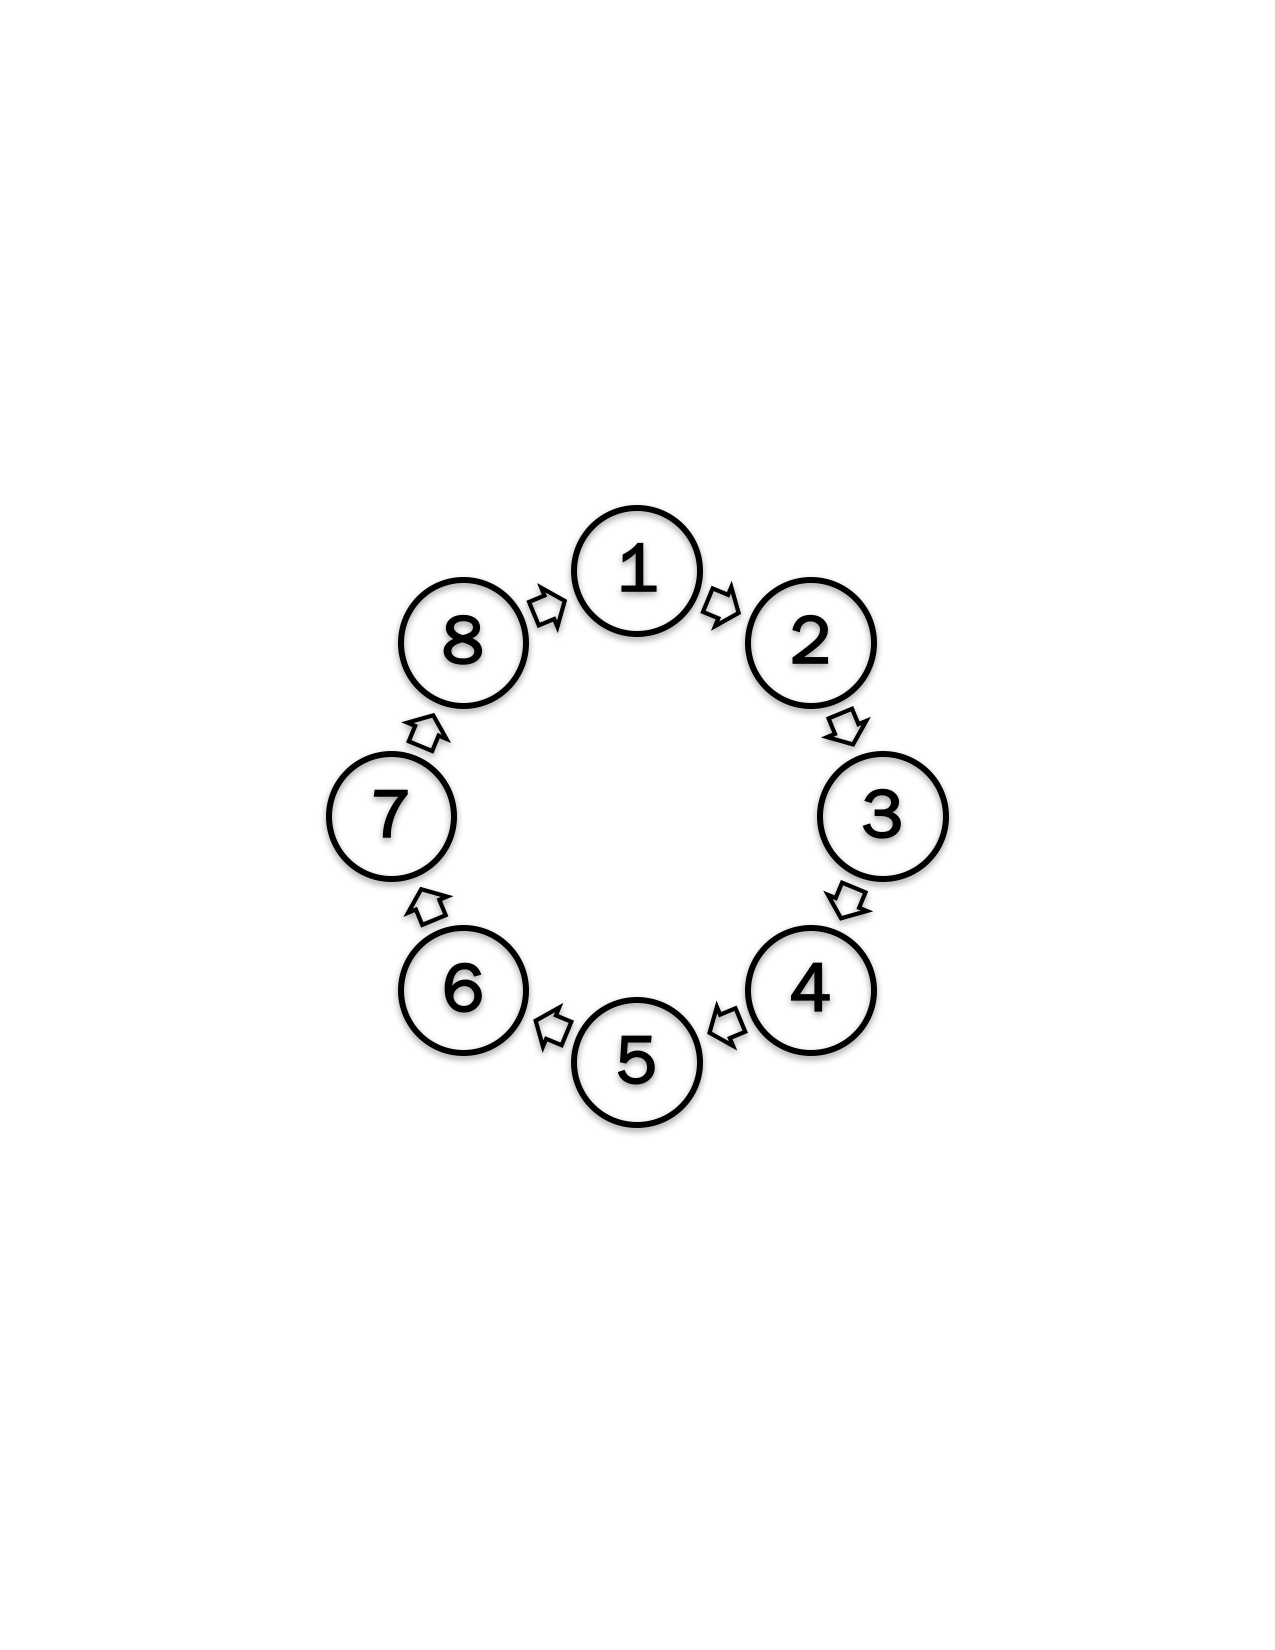
\includegraphics[trim=3cm 8.0cm 3cm 8cm,width=\linewidth]{ring_detector.pdf}
  \captionof{figure}{Ring topology}
  \label{fig:Ring}
\end{minipage}%
\begin{minipage}{.23\textwidth}
  \centering
  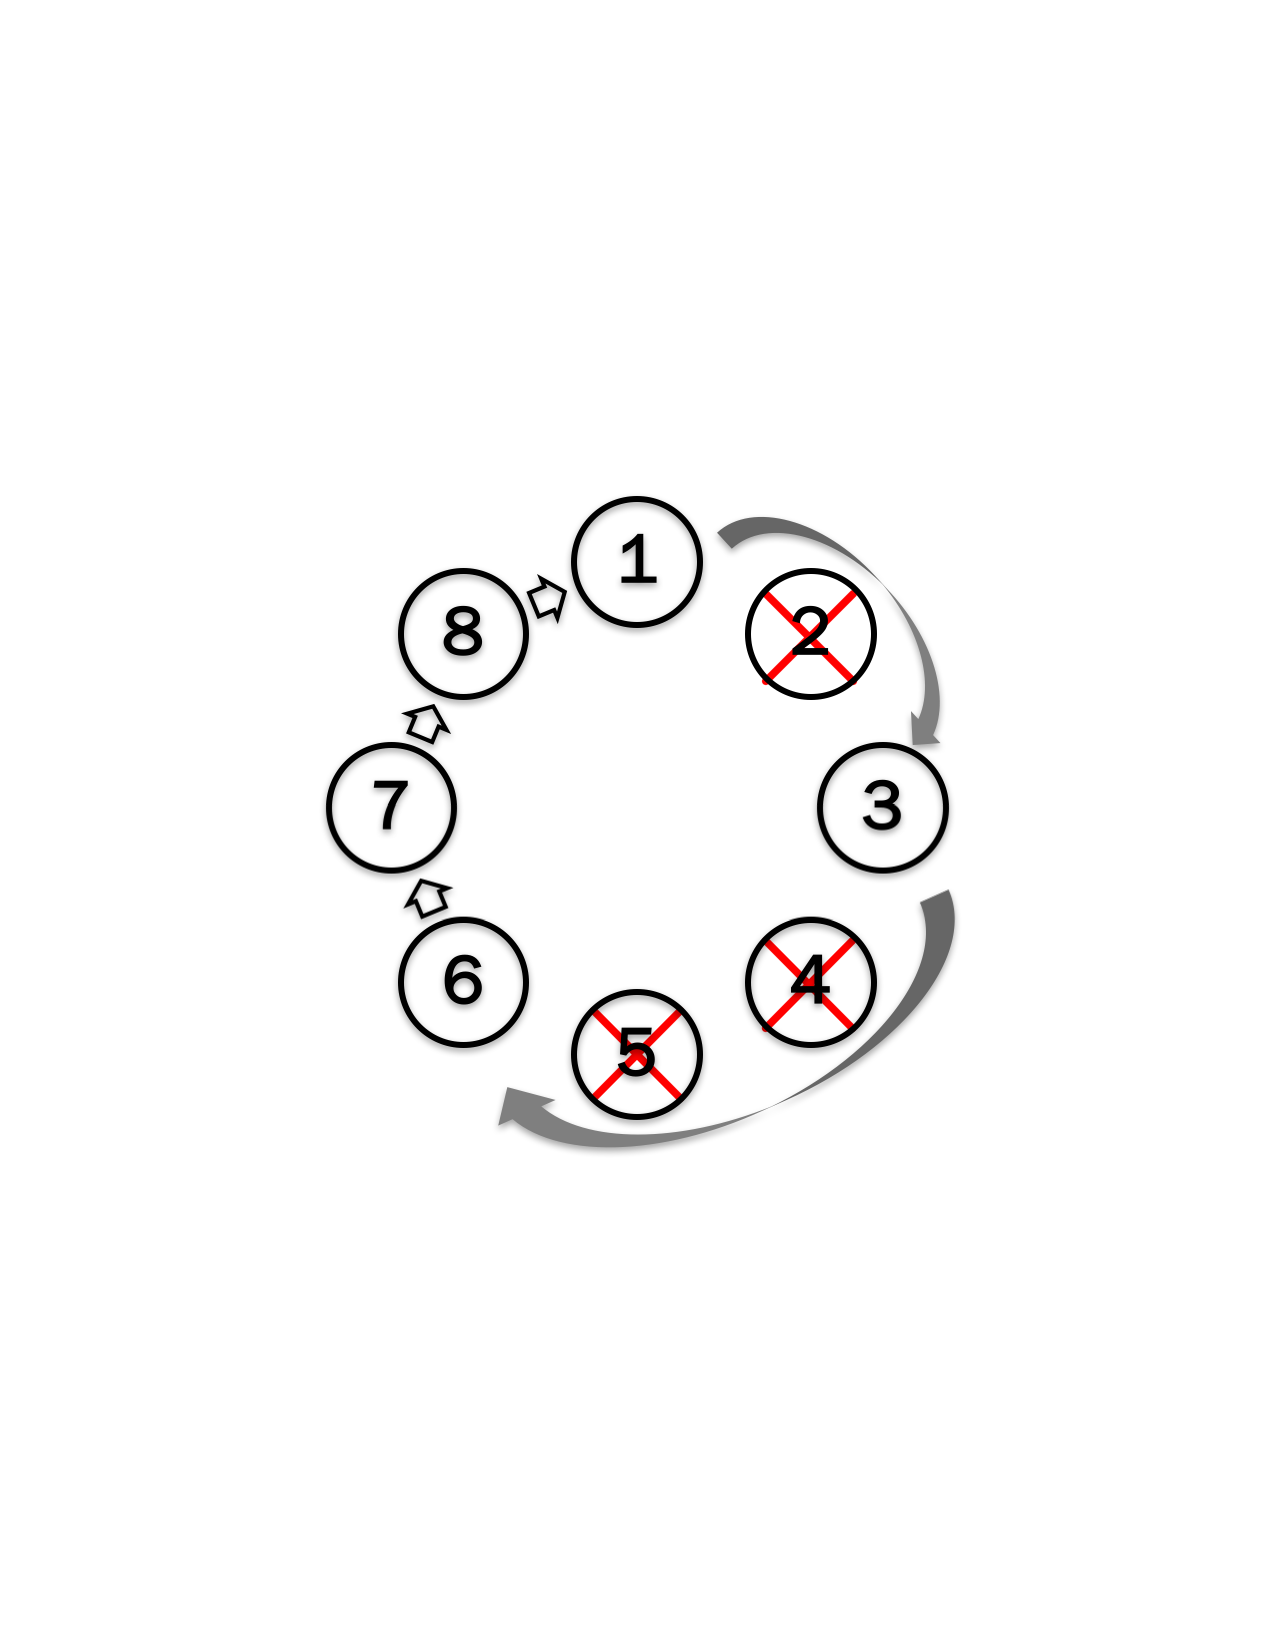
\includegraphics[trim=3cm 8.0cm 3cm 8cm,width=\linewidth]{reconnet_cross.pdf}
  \captionof{figure}{Reconnect with failures}
  \label{fig:Reconnect Ring}
\end{minipage}
\end{figure}
We provide a strategy to detect both process failure and node failure in different ways. The OpenRTE Daemon's Local Launch Subsystem(odls) is responsible for launching and monitoring local processes that are intended to launch the target applications' executable. Before the children processes execute the targets' executable, it need to set affinity of children processes according to a complex series of rules. This binding may fail in a myriad of different ways, the children processes will send a message to the parent indicating what happened (rendered error message) and the parent will read the message and analyze if this is a process failure and then use the runtime system's reporting mechanisms to display this error globally. 

For a general distributed system, nodes can communicate to any other nodes by sending message through communication channels. We arrange all N nodes to a logistic ring topology as in figure 3, which means, each particular node \textbf{\textit{p}} has a observer and a predecessor in the ring. The predecessor will send periodic heartbeat messages to \textbf{\textit{p}} with the period of $\delta$, at the same time \textbf{\textit{p}} will send heartbeat messages to its observer. For each node it emits heartbeats $m_1$, $m_2$, ... at time $\tau_1$, $\tau_2$, ... to its observer \textbf{\textit{q}}. Let $\tau_i' = \tau_i + t$. At any time \textbf{\textit{t}} $\in [\tau_i', \tau_{i+1}')$, \textbf{\textit{q}} believe \textbf{\textit{p}} is alive if it receive message $m_i$ or higher. Otherwise, \textbf{\textit{q}} suspect \textbf{\textit{p}} is failed, \textbf{\textit{q}} will prepare error information of \textbf{\textit{p}} and propagate this information. 

When the observer detects that the predecessor is failed, there are two major steps we do. First we need to reconnect the ring topology as in figure 4, the observer will search its own known failed list and figured out the first alive node \textbf{\textit{nq}} preceding in the ring, it set \textbf{\textit{nq}} as its predecessor and then send a request to \textbf{\textit{nq}} for being the new observer. The second step is failure propagation: the observer need to get access to the job's global mapping and binding information and find out all those processes hosted on predecessor node. After we get the list of all those affected processes and node, the observer calls the propagation component to delivery this message on node level to its neighbours, then observer will notify its local processes. Then, the observer updates its local known failure List\{\textit{ID}\}. For all those nodes who received the notification, each node need to forward this information, maintain its own List\{\textit{ID}\} and notify locally. As show in figure 1, we created a new module in error management as detector to enable this feature.

\subsection{Failure propagation}
For broadcasting we use the scalable and fault tolerant topology binomial graph (BMG)\cite{Angskun07}. BMG has good fault-tolerant properties such as optimal connectivity, low fault-diameter, strongly resilient and good optimal probability in failure cases. In order to continuing the job execution rather than aborting, we need let all participated nodes and applications be aware of failures, the three major mechanisms are 
\begin{enumerate}
  \item Observer fetch error information of failed node. Start the propagation globally by calling group communication component for broadcasting.
  \item Observer node broadcasts the information to all its local children. 
  \item All nodes forwarding the message upon receiving to make the broadcast reliable. Make sure all alive nodes receive the information at least once. 
\end{enumerate}

\begin{algorithm}implementation
\caption{Reliable broadcast algorithm }
\textbf{\textit{N}} \Comment{Number of alive nodes}\newline
\textbf{List\{$EID$\}} \Comment{Local list of known error processes' identifier}\newline
\textbf{\textit{msg}} \Comment{Message packed with jobid, process identifiers and state}\newline
\textbf{\textit{flag}} \Comment{Boolean flag indicating forward the message or not}\newline
\textbf{List\{$AID$\}} \Comment{Processes identifiers' hosted on failed daemon identifier }\newline

\begin{algorithmic}[1]
\Procedure{Broadcast}{ $i, N, msg$ }\Comment{Daemon \textbf{i} send error message to all its neighbours}
\For{ $k \gets 0$ to $\log_2 N$ }\Comment {Order not fixed}            
     \State {\textbf{i} send \textbf{msg} to  ( ($N$ + i + $2^k$) \textbf{mod} {N} ) }
     \State {\textbf{i} send \textbf{msg} to  ( ($N$ + i - $2^k$) \textbf{mod} {N} ) }
\EndFor
\EndProcedure
\end{algorithmic}

\begin{algorithmic}[1]
\Procedure{Forwarding}{ $flag, msg$ }\Comment{Daemon \textbf{j} receives msg, forwarding and notify locally }
\If {$flag == true$}
    \State Broadcast( $j, N, msg$ )
    \State Update \textbf{List\{$EID$\}}
    \State Notify locally
\EndIf
\EndProcedure
\end{algorithmic}

\begin{algorithmic}[1]
\Procedure{Start propagation}{ $job, Eid, state$ }\Comment{Daemon \textbf{j} start propagation }
\If {( $Eid$ $\notin$ List\{$EID$\} )}
    \State Add $Eid$ to $msg$
    \State Get \textit{AID} and adde to $msg$
    \State Broadcast( $j, N, msg$ )
    \State Add $Eid$ \textit{AID} to List\{$EID$\}
\EndIf
\EndProcedure
\end{algorithmic}

\end{algorithm}

Group communication use out-of-band non-blocking peer to peer communicate channel as the basic message exchange mechanism, we assume the communication latency from any two directly connected nodes with same message size are equivalent. For node level broadcast, each node sends message to all its neighbours  as in BMG topology, message from any node we follow the sequence as in binomial spanning tree by which means that any node in BMG can always be delivered within $O(log_2^N)$ steps.

\begin{figure}
  \centering
  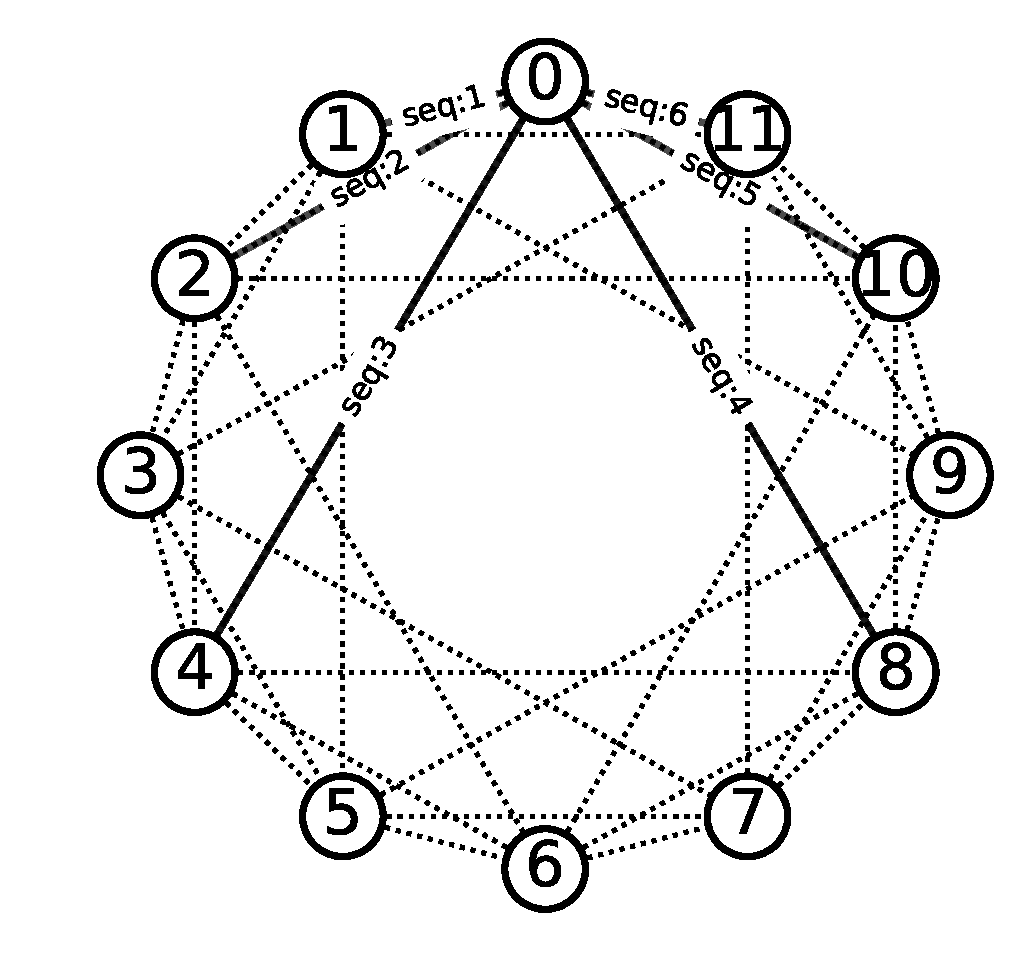
\includegraphics[width=\linewidth]{BMG_seq.pdf}
  \caption{Binomial graph with 12 nodes}
\end{figure}
\begin{figure}
  \centering
  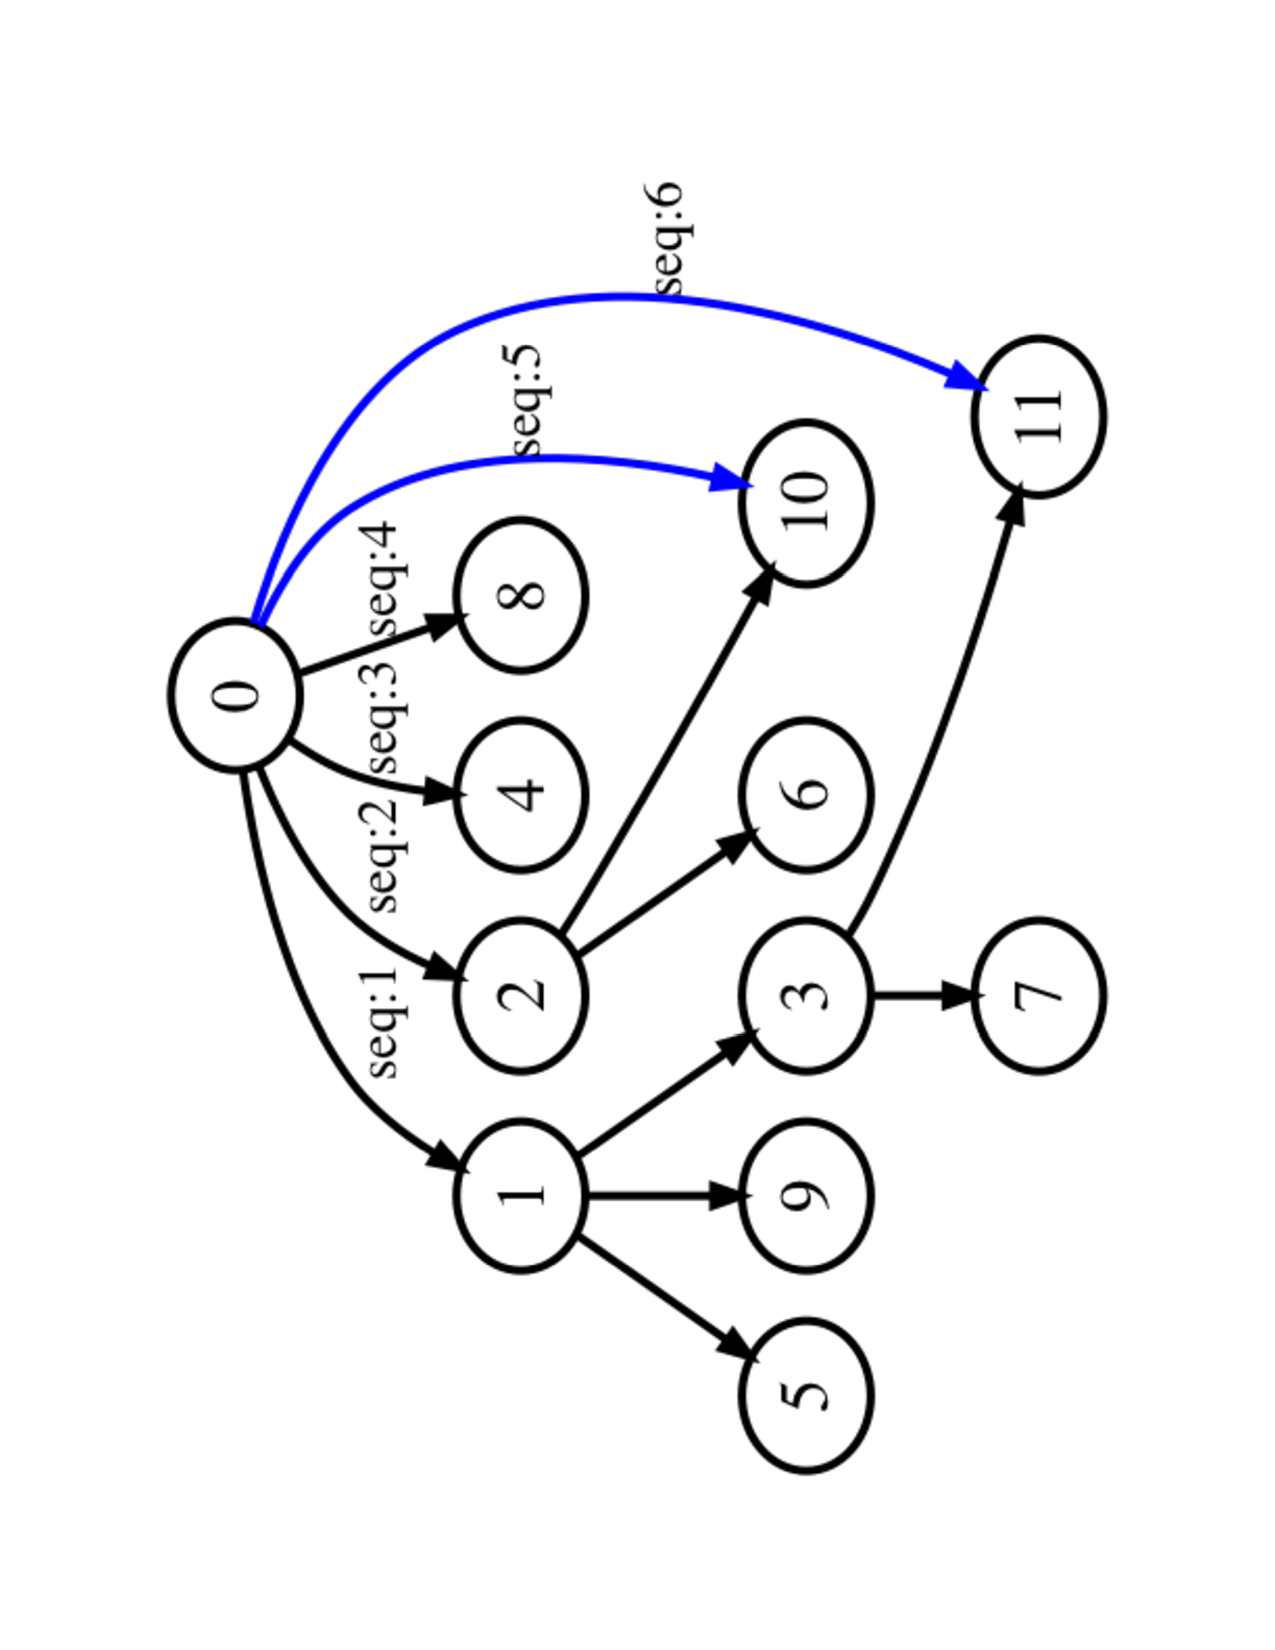
\includegraphics[trim=0.2cm 0.4cm 0.2cm 0.2cm, width=0.9\linewidth,angle=270]{reoder_span.pdf}
  \caption{Broadcast using binomial spanning tree from node 0, extra messages to neighbours are colored in blue }
\end{figure}
Figure 5 shows the BMG with 12 nodes, node 0 starts the propagation and sends messages to all its six neighbours with the sequence marked. And Figure 6 shows the a spanning tree for broadcast originated from node 0 also with extra messages colored blue for resilient purpose. Those extra messages balanced the trade-offs between high-radix trees that allow more parallelism at each level in the tree and more network connections, and lower-radix deeper communication trees with reduced network congestion. The advantages of this new broadcast algorithm are:
\begin{enumerate}
  \item With excellent network connection brings higher parallelism: message to node \{10, 11, 7\} could arrive from any forwarding nodes at earlier time stamp than routed from spanning tree, this decrease the height of the tree, the average latency and the maximum of notification latency are smaller.
  \item With limited network connection: maintains the upper bound of broadcast to $O(log_2^{N})$. 
\end{enumerate}
For inter-node notification, children processes subscribe to a event handler with specific error code and will be triggered by the notification function when a daemon doing the locally notification. Also,applications can register to multiple events which enable the capability to receive notification from different jobs. This attribute is introduced in group communication and propagation component.

\section{Experiment Evaluation}

\subsection{Experiment Setup}
The experiment are conducted on two different machines: (1) a local cluster named NaCl, an Intel Xeon X5660 machine with 66 nodes, 12 cores per node. (2) NERSC's Cori\cite{Cori01} -a Cray XC40 with Intel Xeon "Haswell" processor nodes using Cray "Aries" high speed inter-node network,32 cores per node. The resilient PRRTE is based on PRRTE(\#71ef547), with external PMIx(\#21d7c9). The comparison ULFM is based on(\#77f9157). The experiments is repeated 30 times and we present the average. The benchmark are deployed with one MPI rank per core. 
\subsection{Accuracy and noise}
For the first experiment we want to implore the noise overhead generated by the heartbeat ring detector with different heartbeat period from milliseconds to seconds. We also investigate the accuracy of the detector with different heartbeat period. 

The accuracy experiment is conducted similar to \cite{George18}, the default setting of $ \eta $ and $ \delta $ are $ \eta = \delta * 2 $. If the test is successful (no failure is detected when there is no injection, and all injected failure are correctly detected), then we decrease the heartbeat period and repeat the test until a false positive is reported. We explore detector accuracy with two experiments show false positive behavior on 64 nodes on NaCl: 
\begin{enumerate}
  \item No failure is injected but detector shows a node is gone, which means the observer doesn't receive any heartbeat since last time and timeout is reached. We explore the possible reasons for this result with two tests: (1) Test with no communication but compute-only application, all test succeeds until heartbeat period under 20 msec. (2) Test with IMB benchmark with heavy point-to-point communication and collectives, all tests succeed until the heartbeat period lower than 20 msec as above. We assume that the timeout is neither delayed by communication congestion nor compute pressure. We investigated the problem with smaller job size running on less nodes , it shows a better performance. We find out that daemons need some time to launch the processes when starting the job which caused the false positive. 
  \item No failure is injected and node missed its heartbeat sending deadline. With a reasonable timeout value, all daemons can send heartbeats successfully until $ \delta $ as low as 0.1 msec. 
\end{enumerate}

Based on the results we conclude that the granularity of heartbeat timeout is 40 millisecond limited by the latency for daemons to launch all the application processes. And the granularity of sending heartbeat is 0.1 millisecond.  

\begin{figure*}[h]
\centering
\begin{minipage}{.38\textwidth}
  \centering
  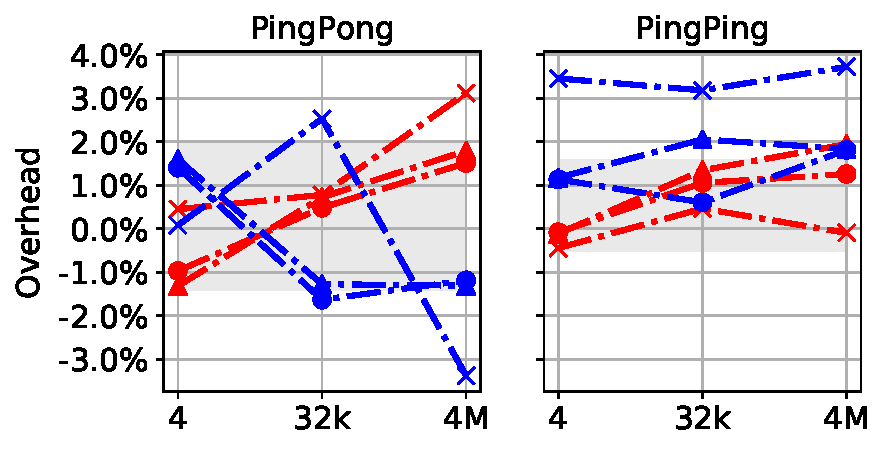
\includegraphics[width=\linewidth]{multi_pingping_pingpong_overhead.pdf}
  \label{fig:Ring}
\end{minipage}%
\begin{minipage}{.62\textwidth}
  \centering
  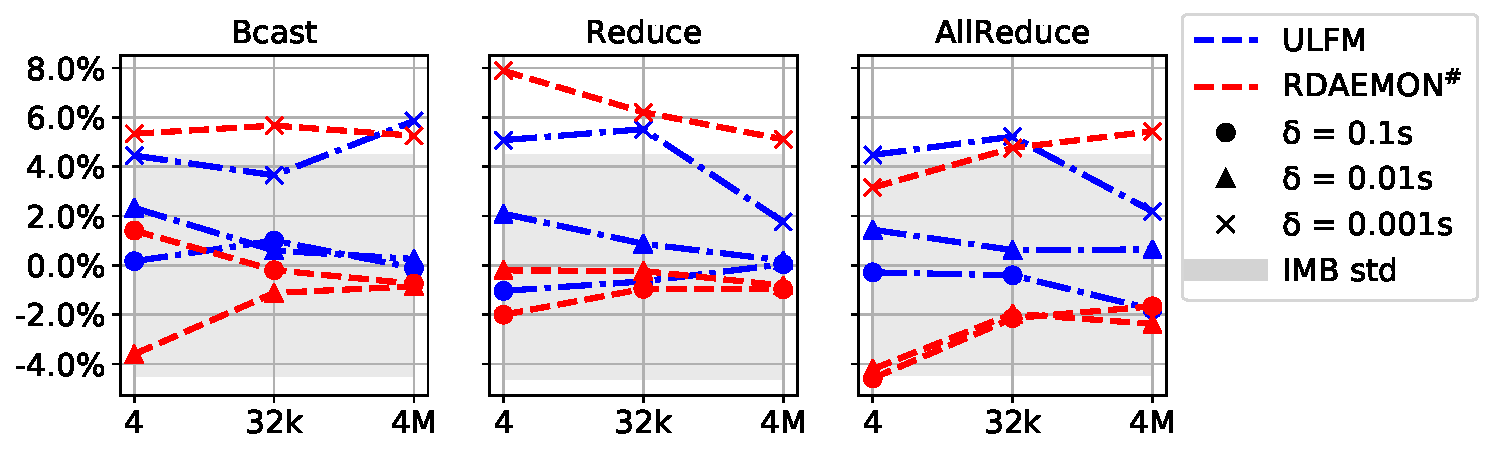
\includegraphics[width=\linewidth]{Bcast_overhead_with_ulfm_max_col.pdf}
  \label{fig:Reconnect Ring}
\end{minipage}
\captionof{figure}{PRRTE with fault tolerance overhead over PRRTE and ULFM using IMB}
\end{figure*}

Figure 7 illustrates the overhead incurred with P2P and collective communications, test results come from Intel MPI benchmark(v2019.2). All IMB-MPI1 suits can be successfully conducted with no false detection with $ \delta \geq 1 ms $. For the P2P setting, we run the benchmark on two nodes will all cores included using the benchmark's "multi" option, which pairs cores from each node as groups to ensure that no matter how daemon are binded to cores the heartbeat emissions affect the performance of P2P communication. For the collective we run the benchmark on 64 nodes using all cores. Any single test we use message size from several bytes to mega bytes, for each message size the test lasts more than 20 seconds to ensure enough heartbeat emissions are occurred during the experiment. The PRRTE overhead is calculated by using the result of benchmark suits (LAT): 
\begin{equation}
\frac{(\ {FT\_PRRTE\_LAT - PRRTE\_LAT}\ )}{PRRTE\_LAT} 
\end{equation}
 From the figure we can see that the latency of performance and bandwidth performance are barely affected by heartbeats with periods from milliseconds to seconds. Notably, point to point communication noise overhead of all tested heartbeats values are less than three percentage. As for collective communication (Bcast Reduce and Allreduce) the noise overhead are less than eight percentage compared to a deviation of four percentage of the benchmark itself. Also we calculated the overhead compared to OpenMPI/ULFM, shows that the overhead results are similar for P2P and collective respectively for all message sizes.

\subsection{Comparison with SWIM}
This section compares failure detection latency and scalability of our failure detector with SWIM\cite{Abhinandan02}, using a random-probing based failure detection protocol and disseminates membership updates via network multi-cast. SWIM uses subgroups to probe to decrease the randomness and increases the scalability. To avoid false detection, SWIM uses suspicion mechanism, when a node does not reply direct or indirect probing in time, the initiator then judges this node as suspicious instead of failure, then broadcasts
\begin{figure}[h]
  \centering
  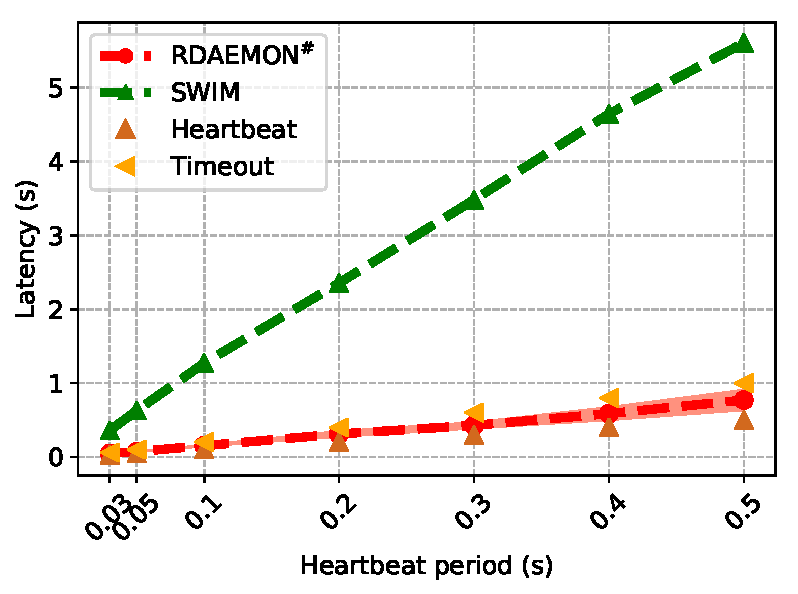
\includegraphics[width=\linewidth]{HB_prrte_swim.pdf}
  \caption{Detection and Propagation delay compared to SWIM using Go-Memberlist}
\end{figure}
this suspicious information within the subgroup, if any node in the subgroup receives an acknowledge before the timeout, it will unmask the suspected node as alive, otherwise mark as failure. In order to improve the efficiency of multi-cast, SWIM uses a infection-style dissemination mechanism as information spreads in a manner analogous to the spread of gossip in society, or epidemic in the general population.

Figure 8 compares detection and propagation latency between our PRRTE detector and SWIM detector of node failure. For the SWIM implementation, we use Go-Memberlist (\#a8f83c6) which is integrated with Go instead of mpi, however we use go-mpi binding to enable SWIM run as mpi application, we use mpi barrier to synchronize before injecting failures in SWIM, and SWIM reports failure through Go-Memberlist callback functions. We run all Memberlist tests only up to 256 processes which is the upper bound of SWIM member limited by maximum connection requests on Transmission Control Protocol (TCP) socket, however this implementation suffers from connection storm and cause consequently crash of continuous running. 

For PRRTE, we also synchronize with barrier, and use our benchmark to inject node failure, detection and notification latency are collected on each process. We run all tests up to 768 processes on 64 nodes.We compare the latency of detection and propagation with different heartbeat period value, for all test we set the timeout equal to two times of heartbeat. We can clearly see that for PRRTE the detection latency is around the middle of heartbeat and timeout between ($\delta$, $2*\delta$), and the receive of notification happens immediately after the detection which demonstrate the efficiency of our propagation algorithm. However for SWIM even with smaller number of processes the delay is still more than $10*\delta$. The variation of PRRTE result comes from the randomness of when the node failure happened.

Figure 9 compare the scalability of the two detectors regard to the number of deployed processes. We set the heartbeat period to 0.5 second with timeout of 1 second. For smaller number of processes PRRTE failure detector is stabilizing in approximately 0.75 second,a statistic behavior of the randomness of when the failure happened between two contiguous heartbeats, while the stabilization delay of SWIM is more than 10 times of heartbeat period. As the number of processes increases, PRRTE's latency remains almost the same. But SWIM shows a linear increase which will be the bottleneck of scaling up(with the assumption it can solve the maximum connection requests limit). For PRRTE with 4K processes the stabilization is still beyond the range of heart period and timeout.

\begin{figure}[h]
  \centering
  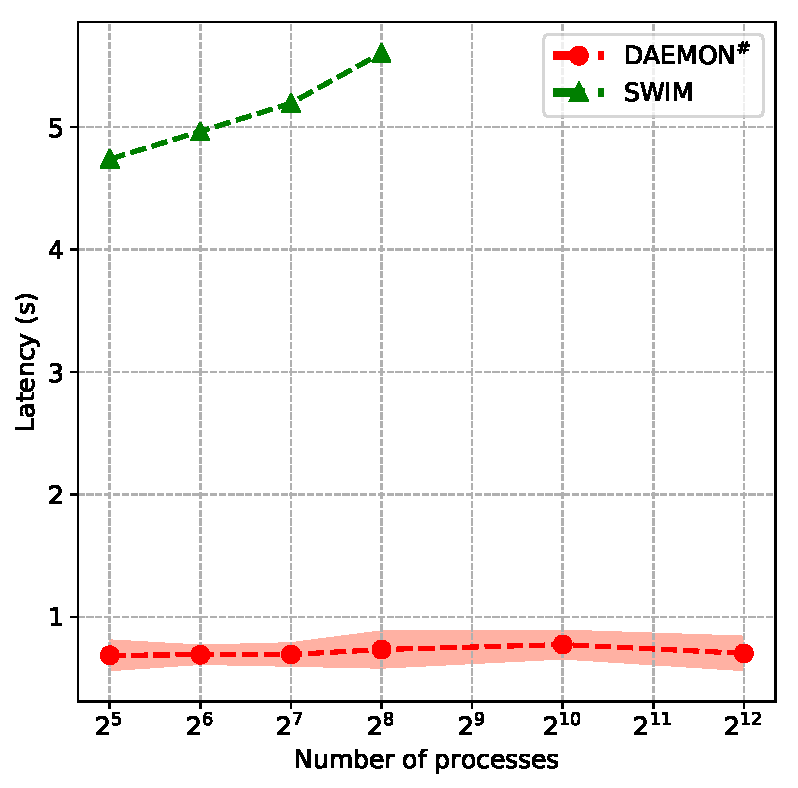
\includegraphics[width=\linewidth]{Scale_prrte_swim.pdf}
  \caption{Scalability compared to SWIM using Go-Memberlist}
\end{figure}

\subsection{Comparison with ULFM for process failure}
This section compares our failure detector with our previous work ULFM\cite{George18}, the ULFM implementation also has two main components: process level detection ring, and propagation overlay with all launched processes. The detection ring is built at Byte Transfer Layer (BTL) level - which provides the portable low-level transport abstraction in OPEN MPI. The current detection implementation provides several mechanisms to ensure the timely activation and delivery of heartbeats:
\begin{enumerate}
  \item Using a separate, library internal thread to send the heartbeats in order to be separated from the application's communication, this also avoid the possible heartbeat delay of compute intensive application. For receiver it need to poll BTL engine to check the aliveness of its successor. 
  \item Using RDMA put to raise a flag in the receiver's registered memory, by using the hardware accelerated put operations solves the problem of active polling BTL engine. 
  \item Using in-band detection for process to report unreachable error directly to the propagation component.
\end{enumerate}

The propagation overlay is also built at BTL level, the small message size of propagation information contains a callback function index which ensures that the received process states update information can be analyzed by upon reception. This method provides independence from the MPI semantic (including matching), however the overlay is constructed with all processes, which means that all participated process need to propagate/forward the error information, the lower bound of reaching any process is bounded by $\log_2({Number\ of\ Processes})$.  

However, PRRTE process failure detection is implemented as the daemons are monitoring the lifeline of all local processes, this mechanism doesn't bring any pressure to the applications' communication resources, also doesn't need RDMA hardware accelerate support. About the propagation strategy of PRRTE, the broadcast overlay is built at daemon level which highly decreases the number of participates, with less participates the total messages transferred and forwarded is much less than the case of ULFM, also the lower bound is $\log_2({Number\ of\ Nodes})$. With the development of more powerful multi-core nodes, the benefit of node level propagation will be much more significant.

\begin{figure}[h]
  \centering
  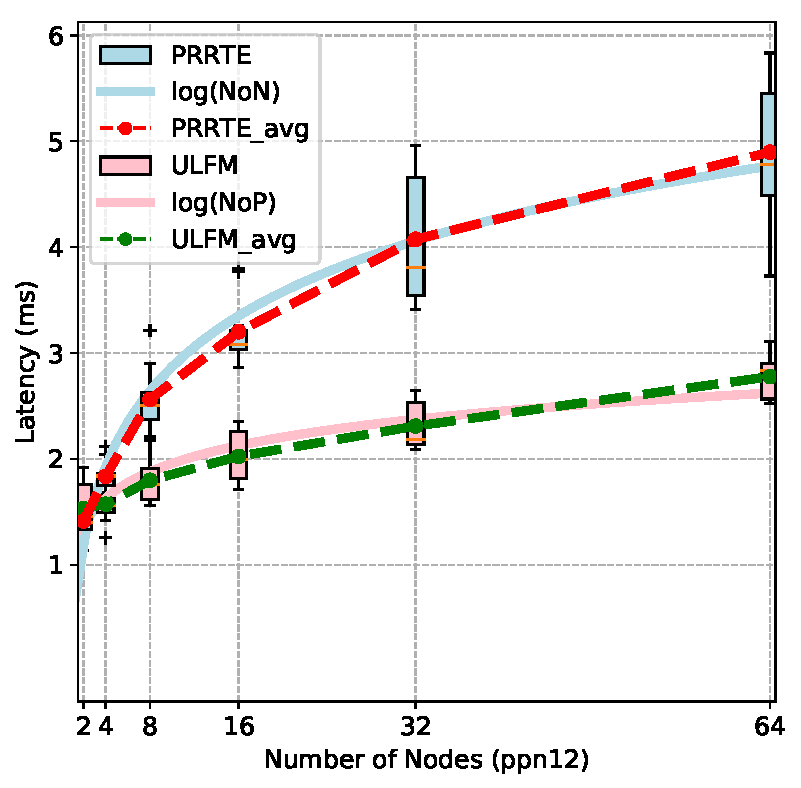
\includegraphics[width=\linewidth]{Process_Failure_log_fit.pdf}
  \caption{Process failure detection and propagation delay compared to ULFM}
\end{figure}

Figure 10 compares the latency of process failure detection and propagation of ULFM and PRRTE. The sensitivity of ULFM heartbeat without false detection is 10 milliseconds, but we want to compare the best performance from ULFM using high speed in-band detection which is faster than using the lowest heartbeat period. For PRRTE, the daemons are in charge of detecting any process failure. PRRTE uses TCP to broadcast among daemons, each daemon uses the PMIx notification method to distribute the error information to all hosted processes. Experiments are conducted on our local cluster NaCl from 2 nodes to 64 nodes using all cores on each node, all processes are equalled mapped to node and bind to core, by doing this ULFM can use the in-band shared communication for detection and propagation. We can see that our implementation gains almost the same performance as ULFM but highly reduced the complexity, the detection and propagation time is less than 5 millisecond with different number of nodes start from 2 to 64 using TCP. For ULFM the detection and propagation delay increase from 2 millisecond to 3 millisecond as the processes number increases with number of nodes using infiniband. For both PRRTE and ULFM the latency increase trend fit to $ a*\log_2(N) + b $, which can be easily scale up to hundreds of thousands of nodes. Similar result strengthens in figure 11 from Cori with more processes on each node, we can see that with 4K processes the detection and propagation latency is about 10 milliseconds. This result indicates the efficiency of our broadcast and propagation algorithm.  

\begin{figure}[h]
  \centering
  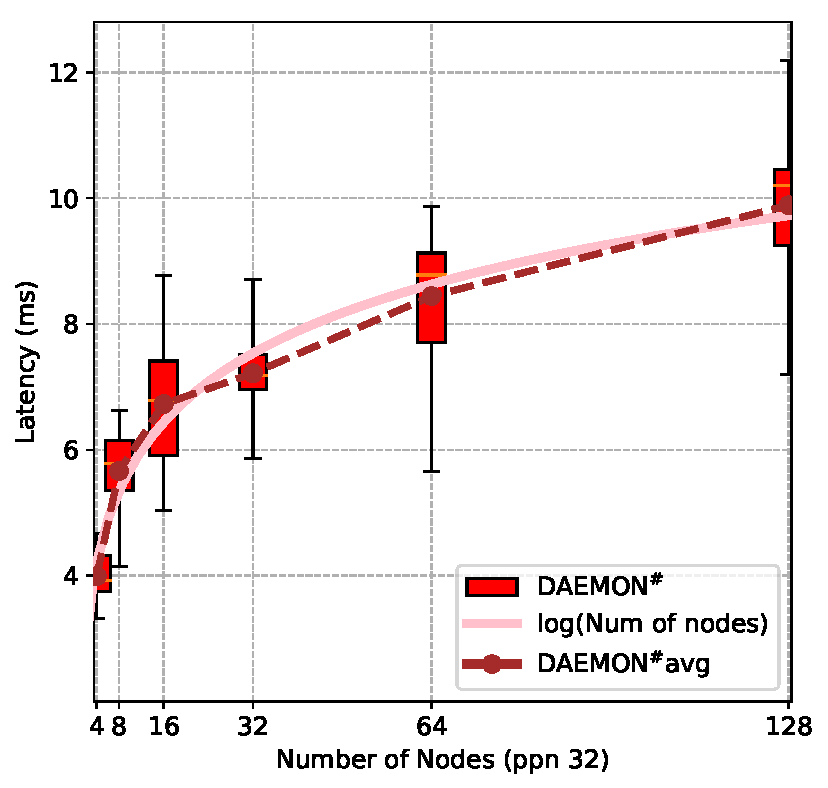
\includegraphics[width=\linewidth]{Cori_Process_Failure_fit.pdf}
  \caption{Process failure detection and propagation delay on Cori}
\end{figure}

\subsection{Node failure detection}
Future more, we want to extend the performance of our heartbeat detector  for node failure detection and propagation from  three perspectives. 
\begin{enumerate}
  \item Latency of detection time and propagation time with different heartbeat periods.
  \item The detection and propagation efficiency using fixed heartbeat and timeout period but with different number of nodes.
  \item Detection latency of multiple node failures.
\end{enumerate}

\begin{figure}[h]
  \centering
  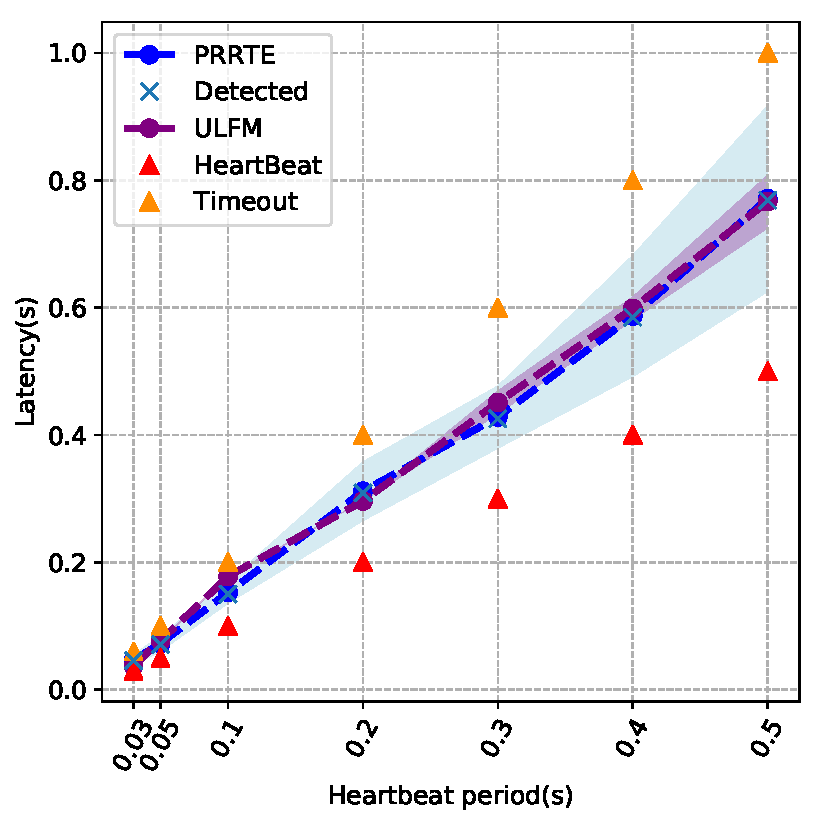
\includegraphics[width=\linewidth]{PRRTE_ULFM_new_nodebug.pdf}
  \caption{Daemon Failure detection and propagation delay compared to ULFM with different heartbeat period}
\end{figure}

Figure 12 presents the behavior observed when injecting single daemon failure under different heartbeat period setting. We conducted the experiments on 64 nodes with 764 processes. For PRRTE after synchronizing, we inject a node crash by choosing a process to kill its host using the parent process identifier. However, ULFM doesn't have the capability of detecting node failure, we simulate "node crash" by kill the last process on that node. With the process ring detector this particular process failure will be detected by its observer on another node, this behavior is the same as PRRTE node to detect node failure. Also we assume that the time different between the daemon failure and process failure is trivial which is confirmed later in the experiment. For the heartbeat period setting we starts at 30 millisecond to 0.5s for both PRRTE and ULFM. For all heartbeat periods we set $ \eta = \delta * 2 $. From the figure we can see that the latency for all cases are bound by $ (\eta - \delta,\eta) $.

Figure 13 shows single node failure detection and propagation performance with fixed heartbeat period $ \delta = 0.5s $ tested with different number of nodes. With a node failure, all processes hosted on this node will be affected, the observer node fetches and packs the information of all affected processes information then distribute the packed message.
\textbf{
\begin{figure}[h]
  \centering
  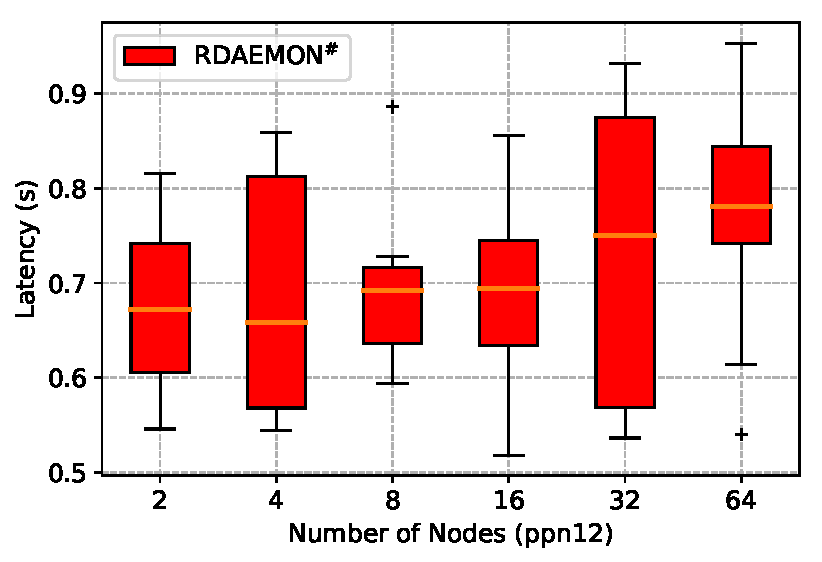
\includegraphics[width=\linewidth]{Daemon_prrte_only.pdf}
  \caption{Daemon Failure Detection and Propagation delay with different number of nodes}
\end{figure}}
However, for ULFM all affected processes need be detected by their observers independently, this will suffer from the collisions on the reliable broadcast propagation. For the worst case, all affected processes are adjacent in the detection ring, for each affected process the ring need to re-connect and update, causes a linear increase of $ \eta $ to the detection latency with every process failure. From the figure see that PRRTE can detect and propagate a node failure between (0.5s, 1s) for all tested number of node. 

The last experiment (Figure 14) investigates the effect of multiple node failures happened in the system. The test setting is the same as single node failure case, except we inject multiple node failures from children processes. For the first scenario, injecting failure to nonadjacent nodes, the detection and propagation are independently conducted by different observer nodes which is a parallel execution. And the results in the figure show that the latency is a constant value which is not affected by the number node failures. The worst scenario is to inject failures to contiguous N nodes, all failures are detected by a single observer (switches to observing the predecessor of the detected failed node). This shows a serial execution. For each node failure it will cause an extra delay of $ \eta $ to the detection latency of the following node failures. From the figure we can see the result matches a linear increase. This extrapolate that from fault tolerance perspective the system will be more stable and reliable by building the detection ring in a arbitrary layout of nodes, avoid choosing predecessor and successor from the same cabinet.  

\begin{figure}[h]
  \centering
  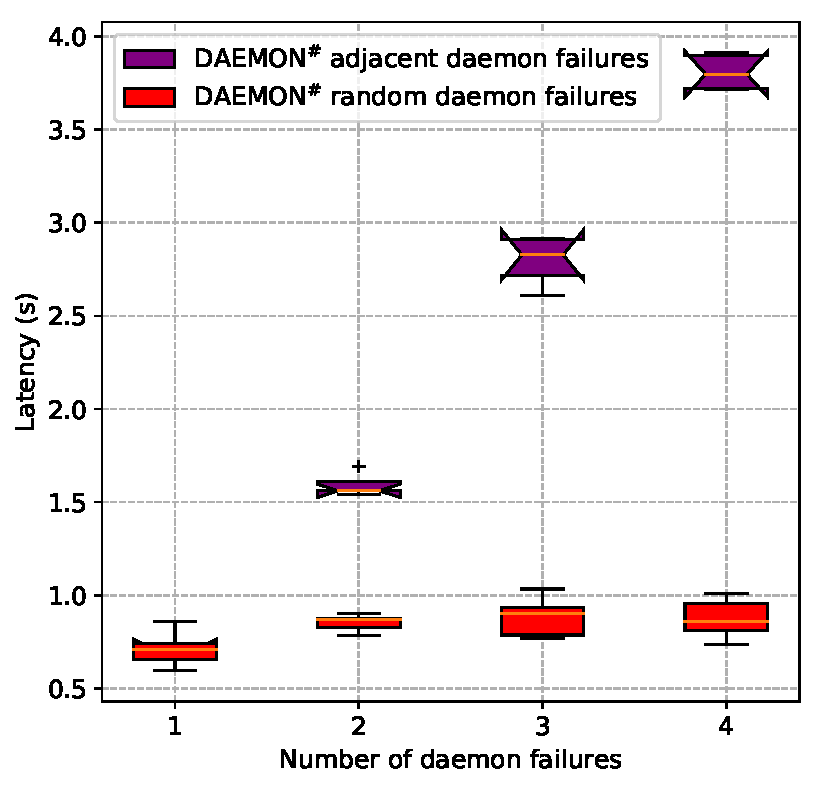
\includegraphics[width=\linewidth]{multi_daemon_failures.pdf}
  \caption{Multiple process failures at the same time}
\end{figure}

\section{Application}
In this section, we present an actual use case of the resilient PRRTE to support the functionality in ULFM of revocation and correction of a broken communicator after node failure. For ULFM the global communicator could be reconfigured after process failure detection, the failed processes are excluded from the global communicator using the MPI\_Comm\_shrink() and are re-spawned using the MPI function MPI\_Comm\_spawn(). However,the job will be aborted with node failure, by using PRRTE instead of OpenMPI runtime the job doesn't need to be terminated after node failure, also with the runtime level propagation mechanism the error message can be delivered to the job scope ( in this case the MPI universe). With the notification MPI application can get the consensus knowledge of failures, then application can use the recovery functions (Shrink, Respawn) provided by ULFM to build new communicator without the processes on the failed node but with those newly spawned processes. 
\todo{add SHMEM, REINIT; thinking about moving this part as 2. Motivation}

OpenSHMEM fault tolerance model is based on check-point and restart, that suits to the one-sided nature of PGAS programming model while leveraging features very specific to OpenSHMEM. Resilient PRRTE failure detection and propagation attributes provide the flexibility to application developers to modulate the frequency and placement within the application where the checkpoint may be introduced. Also the notification provides the trigger for recovery. 

EREINIT a global-restart failure recovery model by allowing a fast re-initialization of MPI. This work is a co-design between MVAPICH and Slurm resource manager to add process and node failures detection and propagation features. The detection is using Slurm's health check mechanism by sending ping messages to nodes, propagation is implemented in a manner of forcing the controller to individually send the notification to children of the failed nodes. However this work is highly depends on one particular resource manager Slurm has the limitation to run only on Slurm machine, also it use a inefficient propagation method. Our resilient PRRTE work can exceed the bottleneck of EREINIT(Slurm machine only) to run on machines with different resource managers. Also with our efficient propagation algorithm the notification will be much faster advances the stabilization and recovery time of EREINIT.

\section{Conclusion}
Failure detection and propagation is a critical service for resilient systems. In this work, we present an efficient failure detection and propagation design and implementation for distributed systems integrated within PMIx\_PRRTE. The process and node failure detection strategy presented in this work depends on heartbeats and timeouts, and communication bound to provide a reliable solution that works at scale without constraints of the kind of faults. Our design and implementation takes into account of the complicate relationship and trade-off between system overhead, detection efficient and risks: low detection time requires frequent emission of heartbeats messages, increasing the system noise and the risk of false positive. Our solution addresses those concerns and capable of tolerating high frequency node and process failures with the help of high performance reliable broadcast notification can quickly disseminate the fault information, our results from different machines and benchmarks compared to two other related work shows that Resilient PRRTE significantly advances the state of art with respect to efficient detection and propagation of failures. This runtime level failure tolerate implementation breaks the limit of running MPI  application only and support all PMIx-based application which is more extensive than MPI scope.   


\section{Acknowledgments}
%
% The acknowledgments section is defined using the "acks" environment (and NOT an unnumbered section). This ensures
% the proper identification of the section in the article metadata, and the consistent spelling of the heading.
\begin{acks}
%CAARES and ECP OMPIX
This material is based upon work supported by the National Science Foundation under Grant No. (1725692); and the Exascale Computing Project (17-SC-20-SC), a collaborative effort of the 
U.S. Department of Energy Office of Science and the National Nuclear Security Administration.    
\end{acks}

%
% The next two lines define the bibliography style to be used, and the bibliography file.
\bibliographystyle{ACM-Reference-Format}
\bibliography{sample-base}

\end{document}
% 
% If your work has an appendix, this is the place to put it.
\appendix
\end{document}
